\chapter{Instalaci\'on de framework Spring en Eclipse Photon y en Luna.}
\textbf{Eclipse Photon :}Lo descargamos de la siguiente p\'agina:\\
\url{http://www.eclipse.org/downloads/packages/}\\
\textbf{Eclipse luna :}Lo descargamos de la siguiente p\'agina:\\
\url{https://www.eclipse.org/downloads/packages/release/luna/r}\\
Descomprimimos el zip ,copiamos la carpeta eclipse en el directorio de archivos de programa, creamos un acceso directo y lo ejecutamos con permiso de administrador.
\begin{figure}[H] 
	\centering
	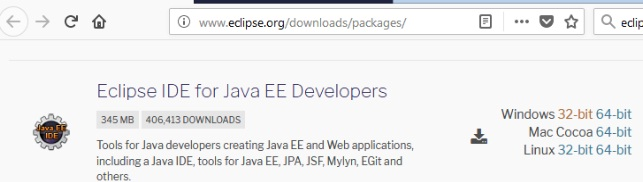
\includegraphics[scale=0.8]{images/c13_1.jpg}
	\caption{P\'agina para descargar Eclipse.}
\end{figure}
\begin{figure}[H] 
	\centering
	
\includegraphics[scale=0.8]{images/c13_2.jpg}
	\caption{Eclipse Photon.}
\end{figure}
\section{Eclipse Photon habilitar marketplace.}
Para que funcione debemos ir a help , Install New Software y agregamos en  el campo Work with :\\
\url{http://download.eclipse.org/mpc/photon}\\
Seleccionamos EPP Marketplace Client  con un checkbox , esperamos su proceso instalaci\'on y despu\'es damos click en finish.Reiniciamos eclipse.
\begin{figure}[H] 
	\centering
	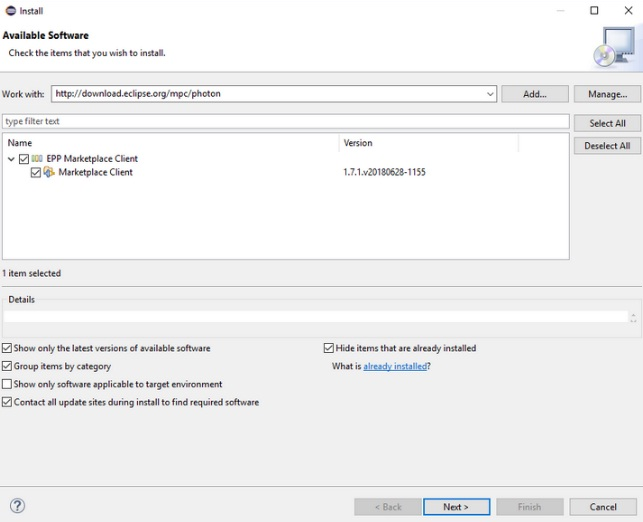
\includegraphics[scale=0.9]{images/c13_3.jpg}
	\caption{Habilitando marketplace.}
\end{figure}
\textbf{Maven :} Ir a help,Install New Software y agregamos en  el campo Work with  : Elegimos All Availables Sites y buscamos maven .Esperamos y elegimos  las dependencias que se muestran en la imagen.
\begin{figure}[H] 
	\centering
	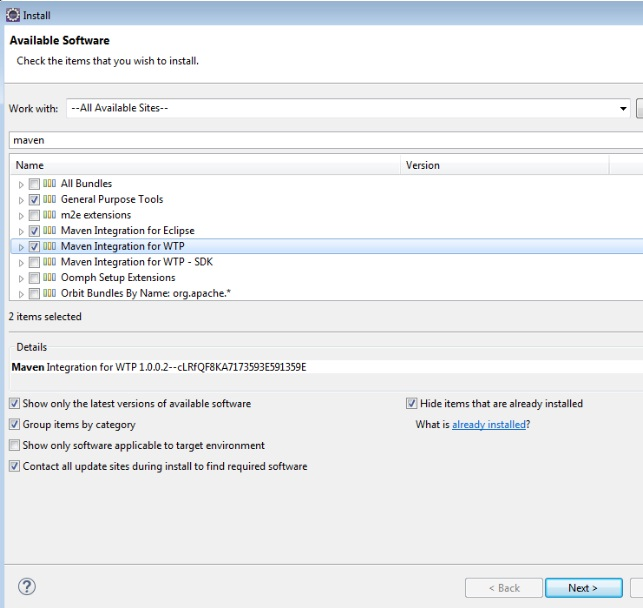
\includegraphics[scale=0.9]{images/c13_4.jpg}
	\caption{Habilitando Maven.}
\end{figure}
\textbf{Spring Tool Suite :} Vamos a help y elegimos eclipse  marketplace.Buscamos  Spring Tool Suite  damos instalar ,click en confirm ,aceptamos los terminos de licencia y esperamos que el proceso de instalaci\'on se termine.
Damos click en finish y reiniciamos Eclipse.
\begin{figure}[H]
	\centering
	\begin{tabular}{c}
		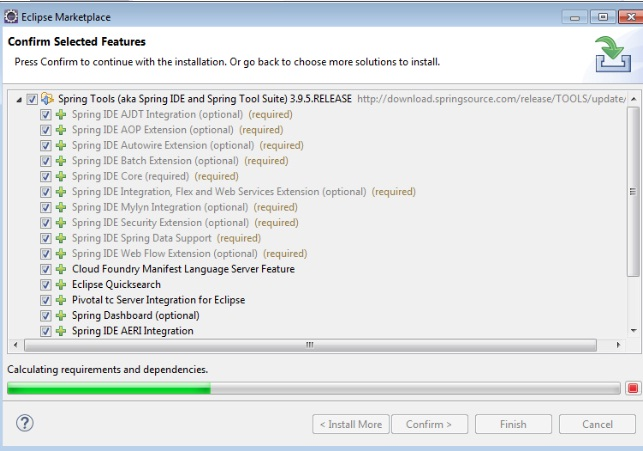
\includegraphics[scale=0.9]{images/c13_5.jpg}\\
		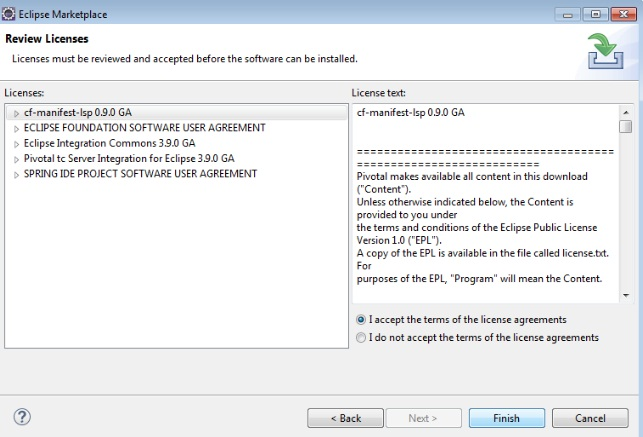
\includegraphics[scale=0.9]{images/c13_6.jpg}
	\end{tabular}
	\caption{Instalando  Spring Tool Suite.}
\end{figure}

\section{Creando nuestro primer proyecto .}
Vamos a File ,new,elegimos Other ,la opcion Java Project,damos click en next,ponemos un nombre al proyecto como ejemplo1 y damos click en finish.	
\begin{figure}[H] 
	\centering
	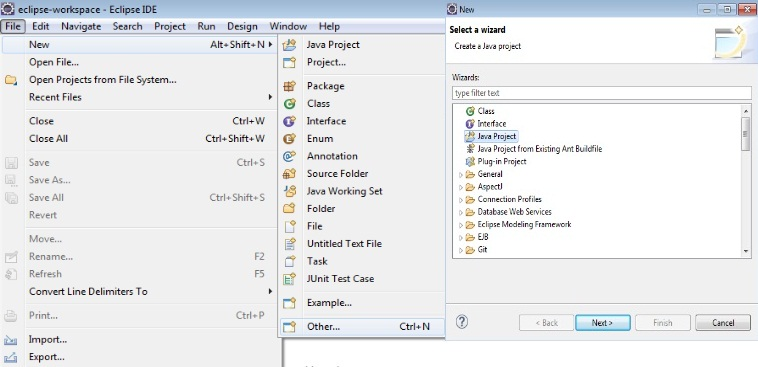
\includegraphics[scale=0.85]{images/c13_7.jpg}
	\caption{Primer Proyecto.}
\end{figure}
\begin{figure}[H] 
	\centering
	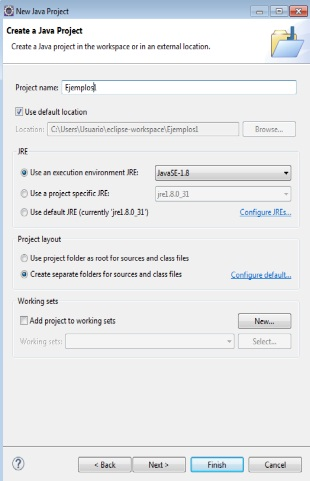
\includegraphics[scale=0.9]{images/c13_9.jpg}
	\caption{Primer Proyecto.}
\end{figure}
En el proyecto damos click derecho elegimos Configure y vamos a la opci\'on Convert to Maven Project y damos click en finish.
Vamos al archivo porn.xml ,en la secci\'on de dependencias damos click en add, agregamos las siguientes dependencias:\\
\textbf{spring-core :} Elegimos el paquete org.springframework y elegimos el jar 4.0.5.RELEASE y damos click en OK.\\
\textbf{spring-beans :} Elegimos el paquete org.springframework y elegimos el jar 4.0.5.RELEASE y damos click en OK.\\
\textbf{spring-context :} Elegimos el paquete org.springframework y elegimos el jar 4.0.5.RELEASE y damos click en OK.\\
\textbf{spring-aop :}Elegimos el paquete org.springframework y elegimos el jar 4.0.5.RELEASE y damos click en OK.\\
\textbf{spring-webmvc :}Elegimos el paquete org.springframework y elegimos el jar 4.0.5.RELEASE y damos click en OK.\\
\textbf{spring-expression :}Elegimos el paquete org.springframework y elegimos el jar 4.0.5.RELEASE y damos click en OK.
\begin{figure}[H]
	\centering
	\begin{tabular}{cc}
		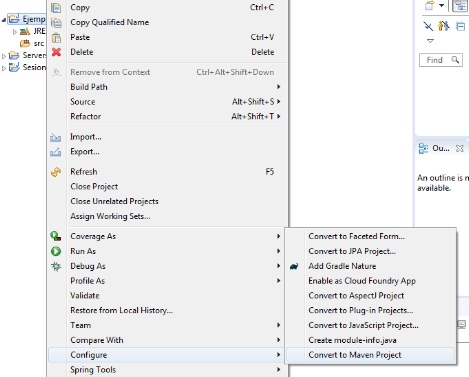
\includegraphics[scale=0.8]{images/c13_10.jpg}
	 &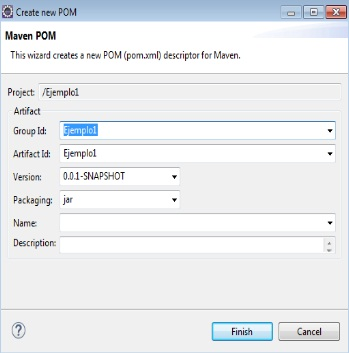
\includegraphics[scale=0.65]{images/c13_11.jpg}
	\end{tabular}
	\caption{Convirtiendo a in proyecto Maven.}
\end{figure}
Tambi\'en lo podemos hacer de forma manual  agregando en el archivo porn.xml despu\'es de la etiqueta </build> ,las dependencias descritas:
\input listaProgramasXML.tex
\begin{pyglist}[caption={porn.xml}]
<dependencies>
<dependency>
<groupId>org.springframework</groupId>
<artifactId>spring-core</artifactId>
<version>4.0.5.RELEASE</version>
</dependency>
<dependency>
<groupId>org.springframework</groupId>
<artifactId>spring-beans</artifactId>
<version>4.0.5.RELEASE</version>
</dependency>
<dependency>
<groupId>org.springframework</groupId>
<artifactId>spring-context</artifactId>
<version>4.0.5.RELEASE</version>
</dependency>
<dependency>
<groupId>org.springframework</groupId>
<artifactId>spring-aop</artifactId>
<version>4.0.5.RELEASE</version>
</dependency>
<dependency>
<groupId>org.springframework</groupId>
<artifactId>spring-web</artifactId>
<version>4.0.5.RELEASE</version>
</dependency>
<dependency>
<groupId>org.springframework</groupId>
<artifactId>spring-webmvc</artifactId>
<version>4.0.5.RELEASE</version>
</dependency>
<dependency>
<groupId>org.springframework</groupId>
<artifactId>spring-expression</artifactId>
<version>4.0.5.RELEASE</version>
</dependency>
</dependencies>
\end{pyglist}


\textbf{Soluci\'on al problema Index downloads are disabled :}
 Vamos a Windows y elegimos Preferences.Vamos a Maven y damos check a las opciones como se muestran en la siguiente figura y damos click en Apply and Close.Y reiniciamos Eclipse.
\begin{figure}[H] 
	\centering
	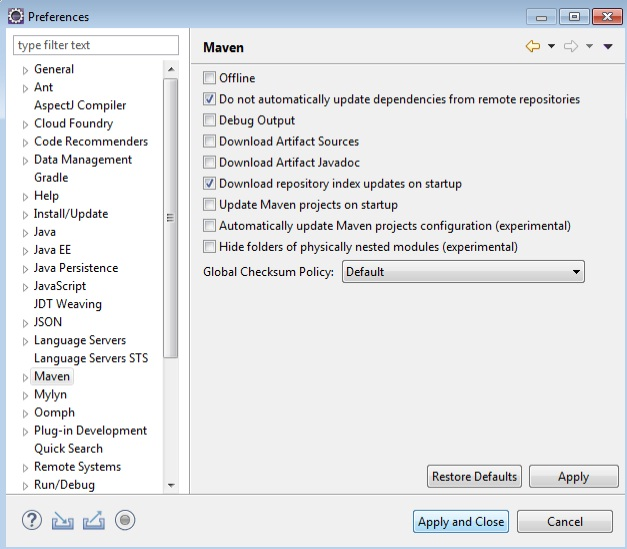
\includegraphics[scale=0.7]{images/c13_12.jpg}
	\caption{Configurando Maven.}
\end{figure}
Ahora vamos  a Windows y elegimos Preferences.Vamos a Maven y elegimos la opcion User Settings .Damos click   en Update Settings y damos  click en Apply and Close. 
Reiniciamos Eclipse.
\begin{figure}[H] 
	\centering
	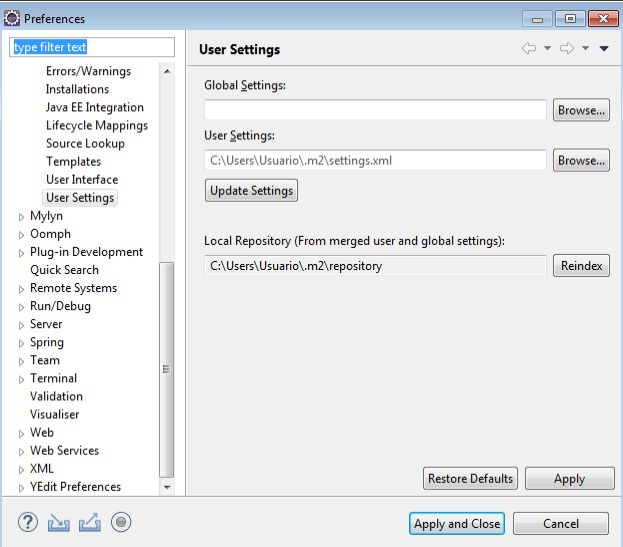
\includegraphics[scale=0.7]{images/c13_13.jpg}
	\caption{Configurando Maven.}
\end{figure}
\subsection{Plain Old Java Object}
\input listaProgramasJava.tex
\begin{pyglist}[caption={Imprimir.java}]
	import javax.swing.*;
	import java.awt.*;
	public class app_prg1 extends JApplet
	{ public void init(){}
		public void paint ( Graphics g ){
			g.drawString(" 3 +46 = "+(3+46),30, 30 );}
	}
\end{pyglist}
\section{}
\section{}